\subsection{Use-case xác thực}
    \begin{figure}[h]
        \centering
        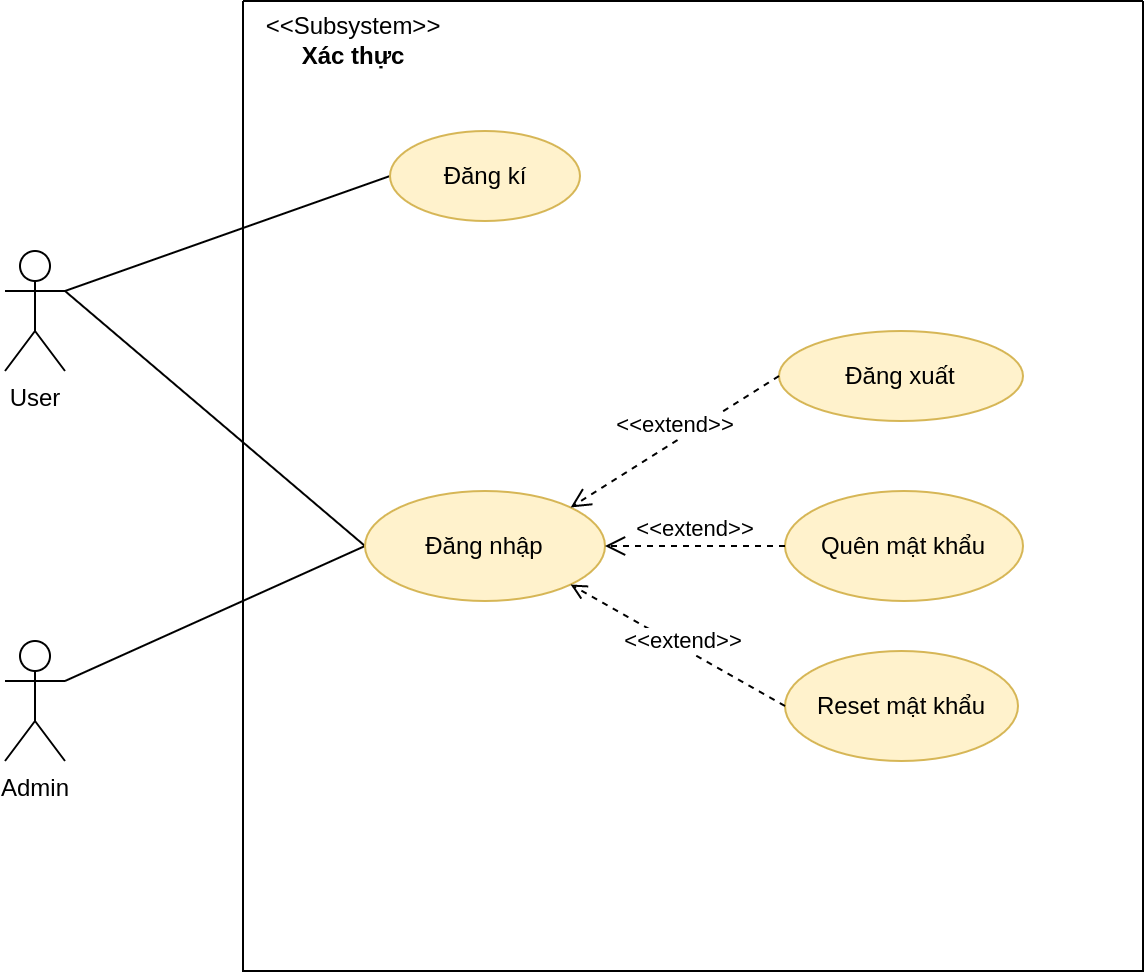
\includegraphics[width=1\linewidth]{images/use-case diagram/authentication_use-case.png}
        \caption{Use-case xác thực}
    \end{figure}

    \begin{tblr}{
        width=1\linewidth,
        hlines,
        vlines,
        colspec={X[3]X[7]},
        columns = {valign = m, },
        row{1} = {halign = c, valign = m, bg = lightgray, fg = black},
    }
        {\textbf{Use case name} & \textbf{Đăng xuất}}  \\
        Description	 & 	Cho phép người hoặc quản lí đăng xuất khỏi hệ thống\\
        Trigger & Cho phép người hoặc quản lí ấn vào đăng xuất \\
        Pre-condition & Đã đăng nhập trên hệ thống \newline
                        Thiết bị có kết nối mạng\\
        Post-condition & Hệ thống ghi nhận đăng xuất thành công \\
        Normal flow &   1. Hệ thống ghi nhận đăng xuất. \newline
                    	2. Tiến hành đăng xuất khỏi thiết bị \newline
                    	3. Quay lại trang chủ \\

    \end{tblr}

    \begin{tblr}{
        width=1\linewidth,
        hlines,
        vlines,
        colspec={X[3]X[7]},
        columns = {valign = m, },
        row{1} = {halign = c, valign = m, bg = lightgray, fg = black},
    }
        {\textbf{Use case name} & \textbf{Đăng nhập}}  \\
        Description	 & 	Người dùng hoặc quản lý đăng nhập vào hệ thống \\
        Actor & Người dùng (User) và quản lý (admin)  \\
        Trigger & 	Người dùng hoặc quản lý ấn vào nút đăng nhập \\
        Pre-condition & Người dùng hoặc quản lý đã có tài khoản \newline
                        Thiết bị có kết nối mạng\\
        Post-condition & Hệ thống ghi nhận đăng nhập thành công\\
        Normal flow &   1. Người dùng hoặc quản lý nhập tên tài khoản và mật khẩu và ấn vào nút đăng nhập \newline
                    	2. Hệ thống truy cập vào database kiểm tra tài khoản và mật khẩu và kiểm tra tài khoản và mật khẩu đã nhập. Nếu hợp lệ chuyển sang bước 3. \newline
                    	3. Cho phép người dùng truy cập vào app với quyền đã được cấp (admin hoặc user) \newline
                    	4. Quay về trang chủ \\

        Exception flow & 	Exception thứ nhất: tại bước thứ 2 nếu tài khoản không hợp lệ thì thông báo tài khoản hoặc mật khẩu sai và yêu cầu nhập lại. \\
       Extension points & Đăng xuất \newline
                        Quên mật khẩu \newline
                        Reset mật khẩu \\
    \end{tblr}

    \vspace{0.7cm}

    \begin{tblr}{
        width=1\linewidth,
        hlines,
        vlines,
        colspec={X[3]X[7]},
        columns = {valign = m, },
        row{1} = {halign = c, valign = m, bg = lightgray, fg = black},
    }
        {\textbf{Use case name} & \textbf{Đăng ký}}  \\
        Description	 & 	Cho phép người dùng mới đăng ký tài khoản \\
        Actor & Người dùng (User)   \\
        Trigger & 	Người dùng hoặc quản lý ấn vào nút đăng ký \\
        Pre-condition & Thiết bị có kết nối mạng\\
        Post-condition & Hệ thống ghi nhận đăng ký thành công và tài khoản được lưu trong database \\
        Normal flow &   1. Người dùng nhập thông tin cần thiết (họ tên, email, ngày sinh, username, mật khẩu) và ấn vào đăng ký \newline
                    	2. Hệ thống kiểm tra thông tin có hợp lệ không \newline
                            - Tên: không bao gồm số và không có kí tự đặc biệt \newline
                            - Email: chỉ chấp nhận email có đuôi @gmail.com \newline
                            - Năm hiện tại - năm sinh > 15 \newline
                            - Username chưa có trong hệ thống \newline
                            - Mật khẩu ít nhất 8 ký tự \newline
                    	3. Hệ thống lưu lại thông tin của người dùng vào database \newline
                    	4. Thông báo cho người dùng đã đăng ký thành công và chuyển sang trang đăng nhập \\

        Exception flow & 	Exception 1: Ở bước 2 nếu sai những thông tin thì yêu cầu nhập lại. \\

    \end{tblr}
    
    \vspace{0.7cm}
    
    \begin{tblr}{
        width=1\linewidth,
        hlines,
        vlines,
        colspec={X[3]X[7]},
        columns = {valign = m, },
        row{1} = {halign = c, valign = m, bg = lightgray, fg = black},
    }
        {\textbf{Use case name} & \textbf{Quên mật khuẩn}}  \\
        Description	 & 	Cho phép người dùng lấy lại mật khẩu khi quên \\
        Actor & Người dùng (User) và quản lý (admin)  \\
        Trigger & 	Người dùng ấn vào quên mật khẩu \\
        Pre-condition & Thiết bị có kết nối mạng\\
        Post-condition & Hệ thống cung cấp lại mật khẩu cho người dùng \\
        Normal flow &   1. Người dùng (hoặc quản lý) nhập vào username hoặc email của tài khoản đã quên mật khẩu \newline
                    	2. Hệ thống kiểm tra username hoặc email có tồn tại trong hệ thống hay không \newline
                    	3. Hệ thống hiển thị ra cho phép người dùng (hoặc quản lý) chọn câu hỏi và câu trả lời bảo mật. \newline
                    	4. Hệ thống kiểm tra câu hỏi và câu trả lời bảo mật có hợp lệ không. \newline
                    	5. Hệ thống hiển thị mật khẩu của người dùng (hoặc quản lý) và quay lại trang đăng nhập \\

        Exception flow & 	Exception 1: Ở bước 2 nếu không tồn tại username hoặc email thì thông báo username hoặc email không tồn tại và yêu cầu nhập lại. \newline
        Exception 2: Ở bước 4 nếu câu trả lời không hợp lệ thì hiển thị không hợp lệ và yêu cầu nhập lại. \newline
        Exception 3: Ở bước 4 nếu nhập thông tin sai quá 3 lần thì tạm khóa chức năng quên mật khẩu trong vòng 5h. \\

    \end{tblr}
    
    \vspace{0.7cm}
    
    \begin{tblr}{
        width=1\linewidth,
        hlines,
        vlines,
        colspec={X[3]X[7]},
        columns = {valign = m, },
        row{1} = {halign = c, valign = m, bg = lightgray, fg = black},
    }
        {\textbf{Use case name} & \textbf{Đổi mật khuẩn}}  \\
        Description	 & 	Cho phép người hoặc quản lí đổi mật khẩu\\
        Trigger & Cho phép người hoặc quản lí ấn vào đổi mật khẩu \\
        Pre-condition & Đã đăng nhập trên hệ thống \newline
                        Thiết bị có kết nối mạng\\
        Post-condition & Hệ thống ghi nhận đổi mật khẩu thành công và mật khẩu phải được đổi trên database \\
        Normal flow &   1. Người dùng (hoặc quản lý) nhập mật khẩu cũ và mật khẩu mới \newline
                    	2. Hệ thống kiểm tra mật khẩu cũ có hợp lệ không \newline
                    	3. Hệ thống kiểm tra mật khẩu mới có đủ 8 kí tự không \newline
                    	4. Thông báo đổi mật khẩu thành công và sửa mật khẩu trên database \\

        Exception flow & 	Exception 1: Ở bước 2 nếu sai mật khẩu thì thông báo sai mật khẩu và chưa thực hiện thay đổi. \newline
        Exception 2: Ở bước 3 nếu mật khẩu không đủ ít nhất 8 kí tự thì yêu cầu nhập lại. \\
    \end{tblr}
    
\newpage